%*******************************************************************************
%*********************************** Third Chapter *****************************
%*******************************************************************************

\chapter{Fine-Grained Image Recognition}\label{chap3}

In this chapter, we provide an overview for Paper \ref{paperA} and \ref{paperB} that focuses on fine-grained image recognition (FGIR)~\cite{wei2021fine} of grocery items. 
Object recognition in grocery shopping scenarios is a challenging task for visually impaired (VI) people~\cite{brady2013visual,cimarolli2012challenges,szpiro2016finding} due to the necessity of visual capabilities to navigate and identify the products. Regarding identifying products, groceries are often structured in fine-grained manners where details on appearance and shape help us to distinguish between different items. However, since distinguishing between packaged items often requires reading text and raw food items can have similar shapes, recognizing fine-grained details can be difficult without the ability to see. 
In recent years, there has been an emerging interest of development of computer vision-based assistive technologies for assisting VIs with grocery shopping~\cite{jafri2014computer,lanigan2006trinetra,winlock2010toward,sosa2017hands,boldu2020aisee,zientara2017third,george2015fine}. Nevertheless, fine-grained recognition of groceries still remain challenging due to the need for real-world training data for such systems to be robust in grocery stores. We aimed to enhance the robustness and predictive performance of image classifiers by combining natural images with external web information with the items. In Paper \ref{paperA}, we have collected a dataset with natural images of groceries with a mobile phone camera, and web-scraped images and text descriptions about the items, for evaluating image classifiers in real-world supermarket scenarios. We perform an ablation study over the different data types in the data set in Paper \ref{paperB}, where we show that utilizing all data types improves the fine-grained classification performance over image classifiers trained with only the natural images. We cover some related work (Section \ref{chap3:sec:related_work}), describe the dataset collection process (Section \ref{chap3:sec:dataset_collection}) and our used approach for utilizing multi-view data (Section \ref{chap3:sec:fgr_of_grocery_items}), as well as summarize the experimental results from the ablation study (Section \ref{chap3:sec:experiments}). 


%This chapter presents an approach for enhancing fine-grained classification performance of grocery items by using web-scraped information. We focus on classification of grocery items due to applicability in assistive vision and its potential to enhance the independence of visually impaired (VI) people [ADD groceries/shopping/object recognition for VI REFs]. Initially, we were interested in learning classifiers with natural images taken in the grocery stores combined with web-scraped information about the grocery items, such as iconic images and text descriptions from supermarket websites. Using iconic images have been used in grocery image classification earlier [ADD grocery paper REFs], however, utilizing text descriptions was as far we know absent for this application even if it has been successfully applied in other image classification problems~\cite{wah2011cub, nilsback2008automated, bujwid2021large}. Thus, we collected our own dataset of grocery items images using a mobile phone camera as well as web-scraped images and text descriptions to study whether this multi-view approaches would benefit training the classifiers (Section \ref{chap3:sec:dataset_collection}). We then select a multi-view learning framework based on the Variational Autoencoder (VAE) for investigating how the different data views affect the fine-grained classification performance (Section \ref{chap3:sec:fgr_of_grocery_items}). 


\section{Related Work}\label{chap3:sec:related_work}

In this section, we will briefly discuss the related work on FGIR, datasets for FGIR, and multi-view learning. 

%\subsection{Fine-Grained Image Recognition}
\vspace{-3mm}
\paragraph{Fine-Grained Image Recognition.} 
The goal with FGIR~\cite{wei2021fine} is to distinguish between a set of visually similar object classes that belong to some super-class. The main challenge is to recognize the fine-grained visual details that are required for discriminating between visually similar objects. In recent years, the successes with deep learning in computer vision have encouraged researchers to explore various approaches for FGIR in different domains with the goal of discriminating between sub-classes of different animals~\cite{van2018inaturalist}, cars~\cite{krause2013stanford_cars}, fruits~\cite{hou2017vegfru}, and retail products~\cite{wei2019rpc}. These approaches can broadly be divided into three directions where the deep networks utilize (i) localization-classification subnetworks, (ii) end-to-end feature encodings, and (iii) external information. 
In (i), the goal is to find parts that are shared across the sub-classes of some general object and then discover how these localized parts differ in appearance. 
This can be achieved by utilizing feature maps from convolutional layers as local descriptors~\cite{zhang2016picking, wang2018learning}, %ding2019selective}, 
employing detection and segmentation techniques for localizing object parts~\cite{branson2014bird,zhang2014part,zhang2016weakly}, 
or leveraging attention mechanisms in scenarios where common object parts are difficult to represent~\cite{fu2017look,zheng2017learning}. %,sun2018multi}. 
With (ii), the goal has been to learn features that are better at capturing local differences by computing second-order feature interactions~\cite{lin2015bilinear,cui2017kernel}, as well as designing novel loss functions~\cite{dubey2018pairwise,chang2020devil}. %dubey2018maximum,dubey2018pairwise,chang2020devil}.
In (iii), data from external domains, such as the web or different modalities (e.g., text or audio), is utilized to influence the learning of fine-grained details in the objects. These additional data types can be relatively cheap to collect and serves as extra guidance for learning useful representations to the FGIR task. The goal with learning from noisy web data is to reduce the need for human-annotated data~\cite{krause2016unreasonable,xu2016webly,sun2019learning}, while learning from multimodal data aims to obtain a joint representation that captures the correspondences between the images and the other modalities~\cite{he2017fine,zhang2018audio,chen2018knowledge}. In addition to FGIR, both web-scraped and multimodal data has been used for zero-shot learning to transfer knowledge from densely annotated categories to learn new fine-grained classes~\cite{reed2016learning,niu2018webly,akata2015evaluation}. Our work in Paper \ref{paperA} and \ref{paperB} is mostly related to (iii) FGIR with external information, where we use web-scraped images and text descriptions in combination with natural images to improve the classification performance of fine-grained grocery recognition.


%The goal with FGIR~\cite{wei2021fine} is to distinguish between images with multiple visually similar sub-categories that belong to a super-category. For example, various attempts have been made to discriminate between sub-categories of different animals~\cite{van2018inaturalist}, cars~\cite{krause2013stanford_cars}, fruits~\cite{hou2017vegfru}, retail products~\cite{wei2019rpc}, etc. The challenge is to recognize differences that are sufficient for discriminating between objects that are generally similar but differ in fine-grained visual details. In recent years, the successes with deep learning in computer vision have encouraged researchers to explore various approaches for FGIR that can broadly be divided into three directions for recognition by utilizing (i) localization-classification subnetworks, (ii) end-to-end feature encoding, and (iii) external information. In (i), the goal is to find object parts that are shared across the sub-categories for discovering details that make the part representations different. This can be achieved by utilizing feature maps from the activations of convolutional layers as local descriptors~\cite{zhang2016picking, wang2018learning, ding2019selective}, employing detection and segmentation techniques for localizing object parts[REFs], or leveraging attention mechanisms when common object parts are difficult to represent or even define [REFs]. With (ii), the goal has been to learn features that are better at capturing subtle and local differences by, for instance, performing high-order features interactions~\cite{lin2015bilinear} as well as designing novel loss functions [Add REFs]. In the third approach (iii), the goal is to leverage external information, for example, web data and multimodal data, in FGIR as additional supervision to the images. We will put more focus on the approach on FGIR with external information next, as we use this approach in Paper \ref{paperA} and \ref{paperB}. 

%\subsection{Recognition with External Information}
%\paragraph{Recognition with External Information.} 
%Learning fine-grained details about objects often requires large amounts of labeled data. To ease the need for large amounts of accurately labeled images, there have been several attempts to let either web-scraped or multimodal data influence learning the fine-grained features of the sub-categories to boost the FGIR performance. Web-scraped images may be noisy in the sense that retrieved images may have high-variations of the objects. For example, the objects of interest can look different in appearance, and there could also be other irrelevant objects in the images that potentially occlude the category to recognize. Hence, incorporating web-scraped data into the training set may establish a domain gap between the easily acquired web data and the original training set which we need to overcome by reducing the domain gap or reducing the negative effects of the noisy web data that can disturb the learning. Another direction than using web-scraped data is to utilize multimodal data, for example, images, text and knowledge bases, for boosting the classification performance. In FGIR, the goal is to establish a joint representation between the images and additional data sources, where the additional data should act like extra guidance for learning useful representations that capture the fine-grained details of objects. Text descriptions have been a popular data type to combine with images, which can be both easy and cheap to collect as they can be accurately generated by non-experts. High-level knowledge graphs of objects have also been used and can contain rich knowledge useful for fine-grained recognition. In addition to FGIR, both web-scraped and multimodal external information has been used for zero-shot learning to transfer knowledge from annotated categories to new fine-grained categories. In Paper \ref{paperA}, we collect web-scraped images and text descriptions of grocery items to accompany real-world images of groceries for FGIR. Then, in Paper \ref{paperB}, we perform a study using multi-view learning to investigate how the external information can enhance the classification performance. Next, we will cover the related work for the multi-view learning approach that we used. 

\vspace{-3mm}
\paragraph{Datasets for Fine-Grained Image Recognition}
There exist many image datasets for benchmarking computer vision models~\cite{deng2009imagenet, nilsback2008automated, wah2011cub, krizhevsky2009learning, lin2014microsoft, van2018inaturalist, massiceti2021orbit, barbu2019objectnet}. These datasets ranges from large-scale datasets annotated by groups of classes, such as~\cite{deng2009imagenet, kuznetsova2020open}, to smaller but densely-annotated datasets~\cite{everingham2010pascal, lin2014microsoft, krishna2017visual, gupta2019lvis}. There also exist domain-specific datasets for FGIR tasks of animals and species~\cite{van2018inaturalist, van2021benchmarking, van2015building, parkhi12a, lampert2009learning}, %~\cite{van2018inaturalist, van2021benchmarking, khosla2011stanforddogs, van2015building, parkhi12a, lampert2009learning}, 
fashion~\cite{liu2016deepfashion, jia2020fashionpedia}, 
airplanes and cars~\cite{vedaldi2014understanding, maji2013fine, krause20133d, gebru2017fine}, %~\cite{vedaldi2014understanding, maji2013fine, krause20133d, yang2015large, gebru2017fine}, 
faces~\cite{parkhi2015deep, huang2008labeled, guo2016ms}, %~\cite{parkhi2015deep, huang2008labeled, cao2018vggface2, guo2016ms}, 
and foods~\cite{hou2017vegfru, bossard2014food}. Several of the mentioned datasets have also been extended to benchmarking in zero/few-shot image classification~\cite{lampert2013attribute, reed2016learning, triantafillou2019meta, bujwid2021large}. 
In computer vision for visually impaired people, we have recently seen an emergence of datasets collected by people who are blind/low-vision~\cite{kacorri2017teachable, gurari2018vizwiz, sosa2017hands, massiceti2021orbit, gurari2019vizwiz}. Datasets for FGIR of grocery items in their natural environments, such as grocery stores, shelves, and kitchens, have been addressed in plenty of previous works~\cite{jund2016freiburg, waltner2015mango, george2014recognizing, merler2007recognizing, geng2018fine, wei2019rpc}. Similarly, there exist other kinds of food datasets with images of various food dishes~\cite{bossard2014food, kawano2014automatic, min2019ingredient}, %~\cite{bossard2014food, kawano2014automatic, min2019ingredient, rich2016towards}, 
cooking videos~\cite{damen2018scaling, damen2021rescaling}, recipes~\cite{marin2019learning, salvador2017learning, yagcioglu2018recipeqa}, and also restaurant-oriented information~\cite{beijbom2015menu, xu2015geolocalized}. Our grocery item dataset (see Section \ref{chap3:sec:dataset_collection}) shares several similarities with the mentioned works above. For instance, all images of raw and packaged groceries are taken in their natural environment, images are taken with a mobile phone camera from an egocentric view-point, grocery classes are hierarchically labeled, and each class have an additional web-scraped iconic image and text description.


\vspace{-3mm}
\paragraph{Multi-view Learning.} 
Machine learning with multiple types of data is an active research field~\cite{baltruvsaitis2018multimodal, xu2013survey}. In particular, the intersection of computer vision and natural language processing has been of great interest and has led to applications such as image captioning~\cite{xu2015show, lu2018neural, aneja2019sequential}, visual question answering~\cite{antol2015vqa, hudson2018compositional, hu2019language}.
In this thesis, we have focused on learning joint representations across different data types by applying the subspace learning approach from multi-view learning~\cite{xu2013survey}. A view can be defined as data that has been recorded from a specific sensor~\cite{salzmann2010factorized}. For example, we consider natural and web images to be from different views as the images have been recorded using different cameras. Subspace learning approaches aims to learn joint representations from multiple views by assuming that each view have been generated from a latent space that is shared among the views. Most methods originate from Canonical Correlation Analysis~\cite{hotelling1936relations} (CCA) where the goal is to linearly project pairs of different views into a lower-dimensional space where the correlation between the projections is maximized. 
There exist various extensions of CCA which uses deep neural networks for learning nonlinear mappings to extract more rich features of the views, such as Deep CCA~\cite{andrew2013deep} and Deep Canonically Correlated Autoencoders~\cite{wang2015deep}. Inspired from the Deep CCA variants, Variational CCA~\cite{wang2016deep} (VCCA) is a multi-view deep generative model that can both learn joint representations and generate new data by sampling from the shared latent space. 
An advantage of VCCA is the straight-forward extension to modeling both a shared latent space and private latent spaces which capture the view-specific variations to focus the learning of shared variations into the shared latent space~\cite{hyvarinen2000independent, salzmann2010factorized, tsai2018learning, wang2016deep, zhang2016inter, damianou2021multi}.
In Paper \ref{paperB}, we employ VCCA, and its extention to private latent spaces, for learning joint representations of the different data views in our grocery item dataset to obtain more robust image classifiers.   


%Especially, there has been many research efforts made in the intersection of computer vision and natural language processing for applications in image captioning~\cite{xu2015show, lu2018neural, aneja2019sequential}, visual question answering~\cite{antol2015vqa, hudson2018compositional, hu2019language}, and learning joint representations with visual and text data~\cite{vedantam2017generative, wu2018multimodal,shi2019variational}. In this thesis, we focus on the latter where we apply ideas from multi-view learning~\cite{xu2013survey} for learning joint representations across data views. A view can be defined as any signal or data measured by some appropriate sensor~\cite{salzmann2010factorized}. A common approach for learning joint representations from multiple views is to assume that each view have been generated from the same latent space shared between all views. An example method is Canonical Correlation Analysis~\cite{hotelling1936relations} (CCA) where the goal is to linearly project pairs of different views into a lower-dimensional space where the correlation between the projections is maximized. There exist various extensions of CCA which uses deep neural networks for learning nonlinear mappings to extract more rich features of the views, such as Deep CCA~\cite{andrew2013deep} and Deep Canonically Correlated Autoencoders~\cite{wang2015deep}. Inspired from the Deep CCA variants, Variational CCA~\cite{wang2016deep} (VCCA) is a multi-view deep generative model that can both learn joint representations and generate new data by sampling from the shared latent space. In the case of noisy views, an advantage of VCCA is that it can be extended to modeling both a shared latent space and private latent spaces for each view which capture view-specific variations to ease the learning of shared variations~\cite{hyvarinen2000independent, salzmann2010factorized, tsai2018learning, wang2016deep, zhang2016inter, damianou2021multi}. In Paper B, we investigate whether the classification performance of grocery items can be improved by extracting the view-specific variations in the web-scraped views by comparing the classification performance of the joint latent representations from standard VCCA and the VCCA-private.

%Learning from combinations of different data sources has been studied frequently in machine learning~\cite{baltruvsaitis2018multimodal, xu2013survey}. Especially, there has been many research efforts made in the intersection of computer vision and natural language processing for applications in image captioning~\cite{xu2015show, lu2018neural, aneja2019sequential}, visual question answering~\cite{antol2015vqa, hudson2018compositional, hu2019language}, and learning joint representations with visual and text data~\cite{vedantam2017generative, wu2018multimodal,shi2019variational}. In this thesis, we focus on the latter where we apply ideas from multi-view learning~\cite{xu2013survey} for learning joint representations across data views. A view can be defined as any signal or data measured by some appropriate sensor~\cite{salzmann2010factorized}. A common approach for learning joint representations from multiple views is to assume that each view have been generated from the same latent space shared between all views. An example method is Canonical Correlation Analysis~\cite{hotelling1936relations} (CCA) where the goal is to linearly project pairs of different views into a lower-dimensional space where the correlation between the projections is maximized. There exist various extensions of CCA which uses deep neural networks for learning nonlinear mappings to extract more rich features of the views, such as Deep CCA~\cite{andrew2013deep} and Deep Canonically Correlated Autoencoders~\cite{wang2015deep}. Inspired from the Deep CCA variants, Variational CCA~\cite{wang2016deep} (VCCA) is a multi-view deep generative model that can both learn joint representations and generate new data by sampling from the shared latent space. In the case of noisy views, an advantage of VCCA is that it can be extended to modeling both a shared latent space and private latent spaces for each view which capture view-specific variations to ease the learning of shared variations~\cite{hyvarinen2000independent, salzmann2010factorized, tsai2018learning, wang2016deep, zhang2016inter, damianou2021multi}. In Paper B, we investigate whether the classification performance of grocery items can be improved by extracting the view-specific variations in the web-scraped views by comparing the classification performance of the joint latent representations from standard VCCA and the VCCA-private.






\section{Dataset Collection}\label{chap3:sec:dataset_collection}


\begin{wrapfigure}{r}{0.37\textwidth}
	%\centering
	\setlength{\fboxsep}{0pt}%
	\setlength{\fboxrule}{1pt}%
	\vspace{-4mm}
	\fbox{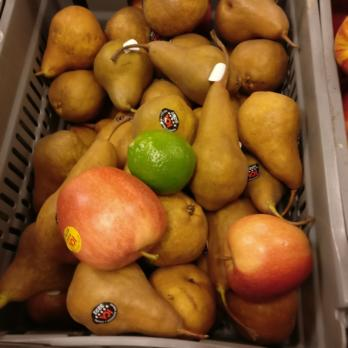
\includegraphics[width=0.15\textwidth]{Chapter3/imgs/Kaiser_029}}%
	~
	\fbox{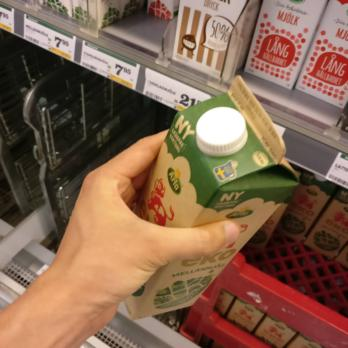
\includegraphics[width=0.15\textwidth]{Chapter3/imgs/Arla-Ecological-Medium-Fat-Milk_011}}%
	\\[4pt]
	\fbox{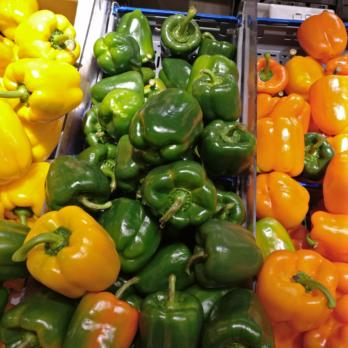
\includegraphics[width=0.15\textwidth]{Chapter3/imgs/Green-Bell-Pepper_020}}%
	~
	\fbox{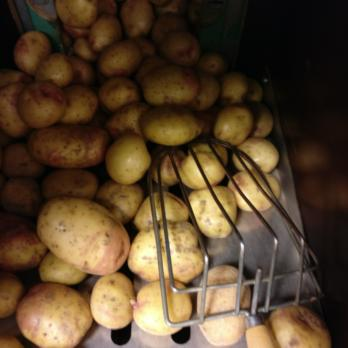
\includegraphics[width=0.15\textwidth]{Chapter3/imgs/Floury-Potato_016}}%
	\vspace{-2mm}
	%\captionsetup{margin={-1mm}}
	\caption{Example images of \\ challenging scenarios.
	}
	\vspace{-3mm}
	\label{fig:example_scenarios_groceries}
\end{wrapfigure} 
In this section, we describe our procedure for collecting the image dataset of grocery items in Paper \ref{paperA}. We visited several supermarkets in Stockholm, Sweden, to collect natural images of groceries with a mobile phone camera to imitate a shopping scenario using an assistive vision device. The collected images captures situations that can be challenging for assistive vision devices, such as misplaced items, hand occlusions, multiple instances and classes present, and various lighting conditions (see Figure \ref{fig:example_scenarios_groceries}). All images were taken with a single targeted item in mind, such that each image is paired with a single label. For items which belong to a clear super-class, e.g., apples and milk packages, we also provided the general class of the items to establish a hierarchical labeling structure of the data. Furthermore, we complemented the image dataset with web-scraped information of each grocery item. More specifically, we visited the online shopping website of a Swedish supermarket chain and downloaded 1) an iconic image of the item on a white background, 2) a text description that describes the flavor and ingredients of the item, and 3) the nutrition values for items where it was applicable. We show four examples of grocery items and their web-scraped information in Table \ref{tab:grocery_store_dataset}. Since these data types are on a class-based level, we can use the web-scraped information as weak supervision to guide the classifier to learn fine-grained details that helps discriminating between visually similar items. We have established training, validation, and test sets of the natural images where the split was made according to the grocery store location to avoid mixing images from different stores. Finally, we made the dataset publicly available under the MIT license\footnote{Grocery Store Dataset URL: \url{https://github.com/marcusklasson/GroceryStoreDataset}}.

%In this section, we describe our procedure for collecting the image dataset of grocery items in Paper \ref{paperA}. As the target use case is grocery shopping with an assistive vision device, we visited several supermarkets and collected natural images of the groceries with a mobile phone camera to imitate such scenarios. Hence, the collected images will capture situations that can be challenging for the assistive device, such as, various lighting conditions, multiple instances and classes present, hand occlusions, and misplaced items. All images were taken with a single targeted item in mind, such that each image is paired with a single label. For items which belong to a clear super-class, for example, various kinds of apples and milk packages, we also provided the general class of the items to establish a hierarchical labeling structure of the data. Collecting natural images of the grocery items is unfortunately a time-consuming process. Furthermore, as the surroundings in every grocery store varies, it may be difficult to build accurate classifiers that can recognize fine-grained details solely from natural images. Hence, we need some cheaper procedure that can complement the collection of real-world images for boosting the classification performance of the groceries. 

%We have complemented the image dataset with external information from the web of each grocery item that can be used for training classifiers. In the past years, most supermarket chains have the option for consumers to purchase groceries online from their websites. The website usually provides each grocery item with an iconic image of the item on a white background, a text description that describes the flavor and ingredients of the item, as well as nutrition values if applicable. We downloaded these information types of all grocery item classes by web-scraping the online shopping website of a supermarket chain. We show four examples of grocery items and their web-scraped information in Table \ref{tab:grocery_store_dataset}. Since these data types are on a class-based level, we can use the web-scraped information as weak supervision to guide the classifier to learn fine-grained details that helps discriminating between visually similar items.   

\begin{table}[t]
	\centering
	\caption{Examples of grocery item classes in the Grocery Store dataset. We display the class label (coarse-grained class in parenthesis), followed by two natural images taken with a mobile phone inside grocery stores, and the %. Next comes 
	the web-scraped information of the items consisting of an iconic image and a text description. We have highlighted ingredients and flavors in the text descriptions that are characteristic for the specific item. }
	\vspace{-10pt}
	\setlength{\fboxsep}{0pt} 
	\setlength{\fboxrule}{0.33pt}
	\resizebox{0.9\textwidth}{!}{
	

	%\resizebox{0.98\textwidth}{!}{
	\begin{tabular}{c | c | c | c}
	\hline
	\thead{\footnotesize Class \\ \footnotesize Labels} & \thead{\footnotesize Natural \\ \footnotesize Images} & \thead{\footnotesize Iconic \\ \footnotesize Images} & \thead{\footnotesize Text \\ \footnotesize Descriptions} \\
	\hline 
	\makecell{ \scriptsize Granny Smith \\[-1pt] \scriptsize (Apple)}
	&  \makecell{ \begin{tikzpicture}
			\begin{scope}
				\node {\fbox{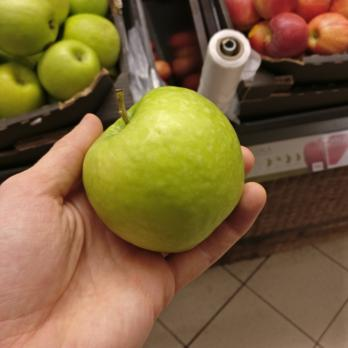
\includegraphics[width=30pt]{Chapter1/pics/Granny-Smith_021.jpg}}};
			\end{scope}
			\begin{scope}[xshift=34pt]
				\node {\fbox{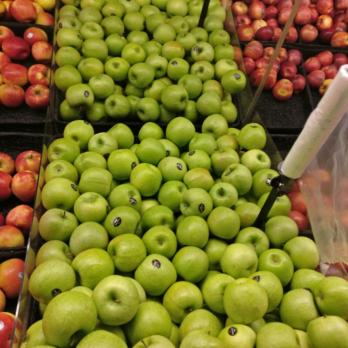
\includegraphics[width=30pt]{Chapter1/pics/Granny-Smith_012.jpg}}};
			\end{scope}
	\end{tikzpicture} }& 
	\makecell{\begin{tikzpicture}
			\begin{scope}
				\node {\fbox{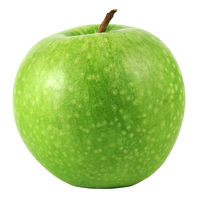
\includegraphics[width=30pt]{Chapter1/pics/Granny-Smith_Iconic.jpg}}};
			\end{scope}
	\end{tikzpicture} } & 
	\begin{scriptsize}
		\makecell{ \textit{“…green apple with white, firm pulp } \\[-1pt]  \textit{and a clear acidity in the flavor.”} } 
	\end{scriptsize}
	\\
	\hline 
	\makecell{ \scriptsize Royal Gala \\[-1pt] \scriptsize (Apple)}
	&  \makecell{ \begin{tikzpicture}
			\begin{scope}
				\node {\fbox{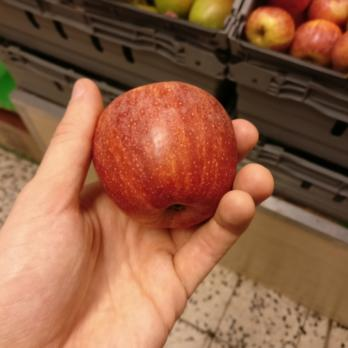
\includegraphics[width=30pt]{Chapter1/pics/Royal-Gala_005.jpg}}};
			\end{scope}
			\begin{scope}[xshift=34pt]
				\node {\fbox{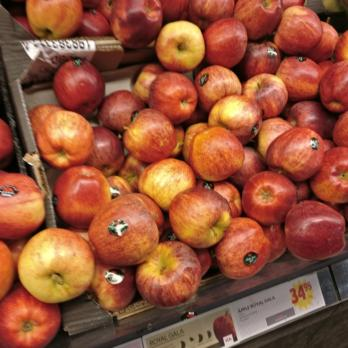
\includegraphics[width=30pt]{Chapter1/pics/Royal-Gala_002.jpg}}};
			\end{scope}
	\end{tikzpicture} }& 
	\makecell{\begin{tikzpicture}
			\begin{scope}
				\node {\fbox{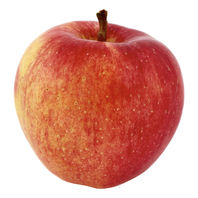
\includegraphics[width=30pt]{Chapter1/pics/Royal-Gala_Iconic.jpg}}};
			\end{scope}
	\end{tikzpicture} } & 
	\begin{scriptsize}
		\makecell{ \textit{“…crispy and very juicy apple,} \\[-1pt] \textit{with yellow-white pulp. The peel} \\[-1pt] \textit{is thin with a red yellow speckled color.”} } 
	\end{scriptsize}
	\\
	\hline
	\makecell{ \scriptsize Tropicana \\[-1pt] \scriptsize Mandarin \\[-1pt] \scriptsize (Juice)}
	&  \makecell{ \begin{tikzpicture}
			\begin{scope}
				\node {\fbox{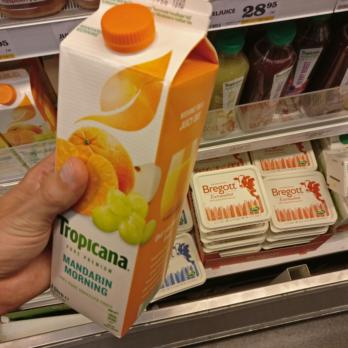
\includegraphics[width=30pt]{Chapter1/pics/Tropicana-Mandarin-Morning_003.jpg}}};
			\end{scope}
			\begin{scope}[xshift=34pt]
				\node {\fbox{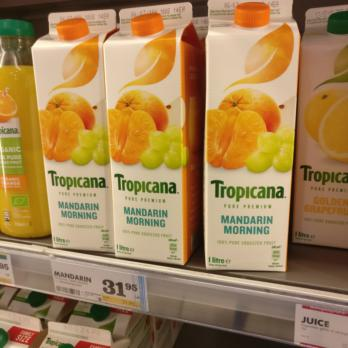
\includegraphics[width=30pt]{Chapter1/pics/Tropicana-Mandarin-Morning_016.jpg}}};
			\end{scope}
	\end{tikzpicture} }& 
	\makecell{\begin{tikzpicture}
			\begin{scope}
				\node {\fbox{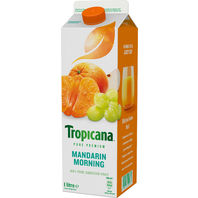
\includegraphics[width=30pt]{Chapter1/pics/Tropicana-Mandarin-Morning_Iconic.jpg}}};
			\end{scope}
	\end{tikzpicture} } & 
	\begin{scriptsize}
		\makecell{ \textit{“…is a ready to drink juice} \\[-1pt]
			\textit{without pulp pressed on orange,} \\[-1pt]
			\textit{ mandarin and grapes. Not from} \\[-1pt]
			\textit{concentrate. Mildly pasteurized.” } }
	\end{scriptsize}
	\\
	\hline
	\makecell{ \scriptsize Yoggi Vanilla \\[-1pt] \scriptsize (Yoghurt)}
	&  \makecell{ \begin{tikzpicture}
			\begin{scope}
				\node {\fbox{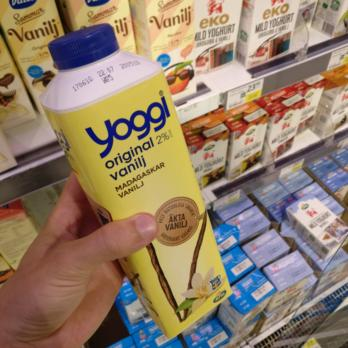
\includegraphics[width=30pt]{Chapter1/pics/Yoggi-Vanilla-Yoghurt_001.jpg}}};
			\end{scope}
			\begin{scope}[xshift=34pt]
				\node {\fbox{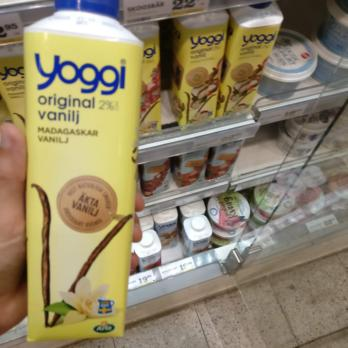
\includegraphics[width=30pt]{Chapter1/pics/Yoggi-Vanilla-Yoghurt_010.jpg}}};
			\end{scope}
	\end{tikzpicture} }& 
	\makecell{\begin{tikzpicture}
			\begin{scope}
				\node {\fbox{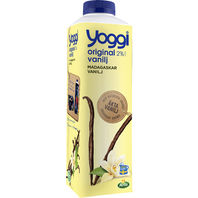
\includegraphics[width=30pt]{Chapter1/pics/Yoggi-Vanilla-Yoghurt_Iconic.jpg}}};
			\end{scope}
	\end{tikzpicture} } & 
	\begin{scriptsize}
		\makecell{ \textit{“...creamy vanilla yoghurt} \\[-1pt]
			\textit{original... added sugar than  } \\[-1pt]
			\textit{regular flavored yoghurt. Great for } \\[-1pt]
			\textit{both breakfast and snacks.”}}
	\end{scriptsize}
	\\
	\hline
\end{tabular}
%}
	}
	\label{tab:grocery_store_dataset}
	\vspace{-2mm}
\end{table}

\section{Fine-Grained Image Recognition of Grocery Items}\label{chap3:sec:fgr_of_grocery_items}

In this section, we describe the problem setting of the grocery item classification task from the dataset collected in Paper \ref{paperA}. Moreover, we describe our approach from Paper \ref{paperB} for learning joint representations of the available data views to improve the classification performance. 

%This section describes the approaches we used for classification of grocery items from the available data types in the collected dataset. We begin by introducing the problem setting, followed by describing the methods for learning representations from the available data views. 

\subsection{Problem Setting}

We focus on the application of training an image recognition app in mobile phones for assisting VIs with grocery shopping. Training such image classifiers typically requires immense amounts of annotated images of the groceries. Additionally, the natural images should be collected in scenarios where the app would be used, such as grocery stores or home environments, which further complicates the collection procedure. To reduce the need for collecting and annotating natural images from mobile phones, we aim to use web-scraped information about the groceries as additional supervision when training the image classifiers. The web-scraped information should help the classifier to focus on learning the learn fine-grained details of the items to improve the classification performance and robustness in real environments. 

%The application we are focusing on is grocery shopping with an assistive vision device. The device could for instance be a mobile phone app where the groceries are recognized by an in-built image classifier from natural images taken with the camera. Training such image classifier to be robust in grocery store environments would typically require an immense amount of labeled training examples of all available groceries. To reduce the need for labeled training data, we aim to combine the collected natural images with web-scraped information about the groceries when training the classifier. The goal is that incorporating the web-scraped information should help the classifier to learn fine-grained details about the items to enhance the classification performance and robustness. 

The following data views are available in the dataset for training the image classifiers:
%The available data views that are available for training image classifiers is denoted as follows:
\begin{itemize}[noitemsep,topsep=1pt]
	\item $\vI$: Natural images of the grocery items taken inside grocery stores.
	\item $\vx$: Feature vectors of the natural images $\vI$ extracted from some CNN $f_{\vvarphi}$ parameterized by $\vvarphi$. 
	\item $\vy$: Class labels of the grocery items in the corresponding natural images.
	\item $\vi$: Iconic images of the grocery items scraped from a supermarket website.
	\item $\vw$: Text description of the grocery items scraped from the same supermarket website as $\vi$.
\end{itemize}
See Table \ref{tab:grocery_store_dataset} for examples of the data views. 
The straightforward approach is to train a CNN with pairs of natural images $\vI$ and class labels $\vy$ in a supervised setting. However, the number of samples may be insufficient for training a CNN from scratch, which can lead to overfitting and low generalization capability to new images. 
One alternative is to employ transfer learning~\cite{zhuang2020comprehensive} where parameters from a CNN pretrained on some large dataset, such as Imagenet~\cite{deng2009imagenet}, are used for initialization and we adapt the network to the grocery item recognition task by either 1) fine-tune some of the final layers, or 2) train a linear classifier from extracted features~\cite{sharif2014cnn}. We take the latter approach and use extracted features for training to mitigate overfitting. Furthermore, we use the web-scraped data views for learning more rich representations of the grocery items that can be used for training more accurate and robust image classifiers, which we present in the next section.


%The simplest approach is to take a standard supervised approach and train a CNN from the natural image and class label pairs. An alternative is leverage from CNNs pre-trained on a large dataset, such as Imagenet~\cite{deng2009imagenet}, and fine-tune the final classification layer to the grocery item recognition task~\cite{sharif2014cnn}. We use ideas from multi-view learning~\cite{xu2013survey} and VAEs~\cite{kingma2013auto} for learning joint representations from the available data views that can be used for training the image classifiers, which we present in the next section.  


\subsection{Multi-View Representation Learning of Grocery Items}

We describe the multi-view learning approach we applied for learning joint representations of grocery items to use for training the image classifiers. More specifically, we employed a deep latent variable model called Variational Canonical Correlation Analysis~\cite{wang2016deep} (VCCA) for learning the joint representations. In the VCCA approach, we assume that the different data views have been generated from the same, shared latent space before they are observed in their original data type. The goal is to obtain joint representations by learning the shared latent space that captures the correspondences across the available views. The joint representations can then be used for training more accurate and robust image classifiers.

Figure \ref{fig:vcca_architecture} shows the network architecture of VCCA %that we 
used in Paper \ref{paperB} for learning the joint representations from all available data views. In this example, we have an input image $\vI$ of a juice package with the fine-grained class label $\vy$ \textit{God Morgon Orange and Red Grapefruit Juice}. We obtain the latent representation $\vz$ by encoding the feature vector $\vx = f_{\vvarphi}(\vI)$ of the input $\vI$ extracted from a CNN $f_{\vvarphi}$ pretrained on Imagenet. In Paper \ref{paperB}, we use a DenseNet~\cite{huang2017densely} architecture as $f_{\vvarphi}$. 
We assume that the latent representation $\vz$ is shared by all available views to establish a more rich representation of the grocery item images by using the each available view as additional supervision to the natural images. 
We capture the correspondences between each view by predicting each view separately using the latent $\vz$ as input to decoder networks that are specific for each view. 
The decoder $p_{\vtheta_{\vx}}(\vx | \vz)$ is an MLP similar to the encoder and outputs a reconstruction $\hat{\vx}$ of the feature vector $\vx$. The decoder $p_{\vtheta_{\vi}}(\vi | \vz)$ is a CNN that predicts the iconic image $\vi$, while the decoder $p_{\vtheta_{\vw}}(\vw | \vz)$ is an RNN predicting the next word in the text description $\vw$. 
We have two options for training the image classifier. The first option is a two-step procedure where we 1) train the VCCA model from all available views except the class labels $\vy$, then 2) train a separate classifier $f_{\vlambda}(\vz)$ on the learned latent representations $\vz$ and the class labels $\vy$. The second option is to learn the classifier simultaneously as the latent space by adding a decoder $p_{\vtheta_{\vy}}(\vy | \vz)$ that predicts the class label $\vy$ from $\vz$.
Note that we only use $\vx$ in the encoder part since the natural images is the only view that is available at test time when predicting the item class of new images taken in the grocery store. In the next section, we perform an ablation study over the available views to analyze how each view affects the fine-grained classification performance.  

%This section describes the approach we took for learning representations of grocery items that are shared across the available data types. We employ a deep latent variable model called Variational Canonical Correlation Analysis~\cite{wang2016deep} (VCCA) for learning the shared representation. The main assumption in VCCA is that each data view have been generated from the same latent space. The goal then is to learn this latent space that captures the correspondences between all views into representations shared across the views for the grocery items. This representation can then be utilized for enhance the learning more accurate classifiers as well as for performing tasks such as synthesis and prediction of novel images. Next, we describe how to enable learning the shared latent space. 

%Capturing variations from each view in the learned representation is performed by predicting the original views from the latent space. To obtain the latent representation, we extract the representation by encoding the natural images with neural network. The extracted representation is then used for predicting each view individually by inputting the representation through separate neural networks. Note that we only use the natural images for extracting the latent representation here since it is the only view that is available at test time when we want to use the learned classifier in the grocery store. We have two options for exploiting the new representation to train classifiers. The first option is to train the classifier with the latent representations after we have learned the latent space as described above. The second option is to train the classifier and learning the latent space simultaneously by adding an additional classifier network predicting the class label with the latent representation as input. 

\begin{figure}[t]
	\centering
	\resizebox{0.95\textwidth}{!}{
		
\tikzset{
	path image1/.style={
		path picture={
			\node at (path picture bounding box.center) {
				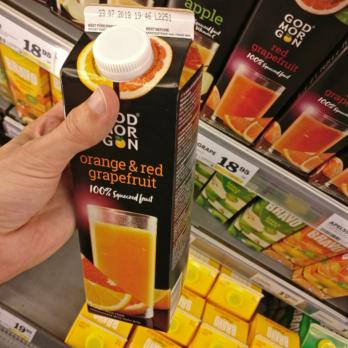
\includegraphics[height=2cm]{Chapter3/tikz/God-Morgon-Orange-Red-Grapefruit-Juice_002.jpg}};}},
	path image2/.style={
		path picture={
			\node at (path picture bounding box.center) {
				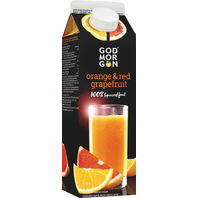
\includegraphics[height=1.5cm]{Chapter3/tikz/God-Morgon-Orange-Red-Grapefruit-Juice_Iconic.jpg}};}},
}

\begin{tikzpicture}
    \node[font=\sffamily] at (1,2.25) {\begin{tabular}{c}Input image $\boldsymbol{I}$ \end{tabular}};
\draw[path image1,draw=black, thick] (0,0) rectangle (2,2);

\node[fill=Green!20, minimum width=0.5cm, minimum height=1.5cm, draw] (x) at (5.25cm,1) {\large $\boldsymbol x$};
\node[font=\sffamily] at (5.25cm,2.25) {\begin{tabular}{c}Feature vector $\boldsymbol{x}$ \\ of image $\boldsymbol{I}$ \end{tabular}};

\draw[fill=orange!20] ([xshift=-0.5cm]x.north west) -- ([xshift=-2.5cm,yshift=1.0cm]x.west) -- ([xshift=-2.5cm,yshift=-1.0cm]x.west) -- ([xshift=-0.5cm]x.south west) -- cycle;
\node at (3.5,1.25) {{\sf \textbf{Pretrained}}};
\node at (3.5,0.75) {{\sf \textbf{CNN} $f_{\boldsymbol{\varphi}}(\boldsymbol{I})$}};

\draw[fill=Green!20] ([xshift=0.5cm]x.north east) -- ([xshift=2.5cm,yshift=0.25cm]x.east) -- ([xshift=2.5cm,yshift=-0.25cm]x.east) -- ([xshift=0.5cm]x.south east) -- cycle; 
\node at (7.0,1.0) {\large $q_{\boldsymbol{\phi}}(\boldsymbol{z} | \boldsymbol{x})$};

\node[fill=red!20, minimum width=0.5cm, minimum height=0.75cm, draw] (z) at (8.75cm,1.0) {\large $\boldsymbol z$};


\node[fill=blue!20, minimum width=0.5cm, minimum height=1.5cm, draw] (xhat) at (12.25cm,1) {\large $\boldsymbol{\hat{x}}$};
\node[font=\sffamily] at (14.25cm,1) {\begin{tabular}{c}Feature vector $\boldsymbol{\hat{x}} \approx \boldsymbol{x}$ \\ of image $\boldsymbol{I}$ \end{tabular}};


\draw[fill=blue!20] ([xshift=0.5cm]z.north east) -- ([xshift=-0.5cm,yshift=0.75cm]xhat.west) -- ([xshift=-0.5cm,yshift=-0.75cm]xhat.west) -- ([xshift=0.5cm]z.south east) -- cycle; 
\node at (10.5,1.0) {\large $p_{\boldsymbol{\theta_x}}(\boldsymbol{x} | \boldsymbol{z})$};

\draw[path image2,draw=black, thick] (12,2.25) rectangle (13.5,3.75);

\draw[fill=blue!20] ([xshift=0.5cm,yshift=2.cm]z.north east) -- ([xshift=2.5cm,yshift=2.75cm]z.east) -- ([xshift=2.5cm,yshift=1.25cm]z.east) -- ([xshift=0.5cm,yshift=2.cm]z.south east) -- cycle; 
\node at (10.5,3.0) {\large $p_{\boldsymbol{\theta_i}}(\boldsymbol{i} | \boldsymbol{z})$};

\node[font=\sffamily] at (14.75cm,3) {\begin{tabular}{c}Iconic image $\boldsymbol{i}$\end{tabular}};

\node[draw,text width=5.25cm,font=\sffamily\itshape] (text) at (14.75cm,-1) {\small{"God Morgon Orange/Red Grapefruit is a fresh blend of sweet orange juice and tasty fresh red grapefruit."}};
\draw[fill=blue!20] ([xshift=0.5cm,yshift=-2.cm]z.north east) -- ([xshift=2.5cm,yshift=-1.25cm]z.east) -- ([xshift=2.5cm,yshift=-2.75cm]z.east) -- ([xshift=0.5cm,yshift=-2.cm]z.south east) -- cycle; 
\node at (10.5,-1.0) {\large $p_{\boldsymbol{\theta_w}}(\boldsymbol{w} | \boldsymbol{z})$};
\node[font=\sffamily] at (14.5cm,-0.1) {\begin{tabular}{c}Text description $\boldsymbol{w}$\end{tabular}};

\node[draw,text width=3.75cm,font=\sffamily] (label) at (14.cm,-3.) {God Morgon Orange and Red Grapefruit Juice};
\draw[fill=blue!20] ([xshift=0.5cm,yshift=-4.0cm]z.north east) -- ([xshift=2.5cm,yshift=-3.25cm]z.east) -- ([xshift=2.5cm,yshift=-4.75cm]z.east) -- ([xshift=0.5cm,yshift=-4.0cm]z.south east) -- cycle; 
\node at (10.5,-3.0) {\large $p_{\boldsymbol{\theta_y}}(\boldsymbol{y} | \boldsymbol{z})$};
\node[font=\sffamily] at (14.cm,-2.3) {\begin{tabular}{c}Class label $\boldsymbol{y}$\end{tabular}};

% Softmax classifier
\node[draw,text width=3.75cm,font=\sffamily] (label1) at (5.75cm,-3.) {God Morgon Orange and Red Grapefruit Juice};
\node[fill=red!20, minimum width=0.5cm, minimum height=0.75cm, draw] (z1) at (1.0cm,-3) {\large $\boldsymbol z$};
\draw[fill=orange!20] ([xshift=0.5cm]z1.north east) -- ([xshift=2.cm,yshift=0.75cm]z1.east) -- ([xshift=2.cm,yshift=-0.75cm]z1.east) -- ([xshift=0.5cm]z1.south east) -- cycle; 
\node at (2.5,-3) {\large $f_{\boldsymbol{\lambda}}(\boldsymbol{z})$};
\node[font=\sffamily] at (5.75cm,-2.3) {\begin{tabular}{c}Class label $\boldsymbol{y}$\end{tabular}};

\draw[draw=black, thick, rounded corners, dashed] ([xshift=-0.5cm,yshift=0.75cm]z1.north west) -- ([xshift=7.5cm, yshift=0.75cm]z1.north west) -- ([xshift=7.5cm,yshift=-0.75cm]z1.south west) -- ([xshift=-0.5cm,yshift=-0.75cm]z1.south west) -- cycle;
\node[text width=8cm,font=\sffamily] at (4.5,-1.6) {Clf. Option 1: Train separate classifier $f_{\boldsymbol{\lambda}}$ with $\boldsymbol{z}$};

\draw[draw=black, thick, rounded corners, dashed] ([xshift=-3.1cm,yshift=0.5cm]label.north west) -- ([xshift=4.5cm, yshift=0.5cm]label.north west) -- ([xshift=4.5cm,yshift=-0.5cm]label.south west) -- ([xshift=-3.1cm,yshift=-0.5cm]label.south west) -- cycle;
\node[text width=8cm,font=\sffamily] at (13.2,-4.3) {Clf. Option 2: Add class label decoder $p_{\boldsymbol{\theta_y}}(\boldsymbol{y} | \boldsymbol{z})$};

% Add edges
\draw[-stealth] (x.east) -> ([xshift=0.5cm]x.east);
\draw[-stealth] ([xshift=-0.5cm]x.west) -> (x.west);
\draw[-stealth] ([xshift=-3.0cm]x.west) -> ([xshift=-2.5cm]x.west);

\draw[-stealth] ([xshift=-0.5cm]z.west) -> (z.west);
\draw[-stealth] (z.east) -> ([xshift=0.5cm]z.east);
\draw[-stealth] ([xshift=-0.5cm]xhat.west) -> (xhat.west);
\draw[-stealth] ([xshift=0.25cm]z.east) -- ([xshift=0.25cm,yshift=2cm]z.east) |- ([xshift=0.5cm,yshift=2cm]z.east);
\draw[-stealth] ([xshift=2.5cm,yshift=2cm]z.east) -> ([xshift=3.0cm,yshift=2cm]z.east);
\draw[-stealth] ([xshift=0.25cm]z.east) -- ([xshift=0.25cm,yshift=-2cm]z.east) |- ([xshift=0.5cm,yshift=-2cm]z.east);
\draw[-stealth] ([xshift=2.5cm,yshift=-2cm]z.east) -> ([xshift=3.0cm,yshift=-2cm]z.east);
\draw[-stealth,dashed] ([xshift=0.25cm,yshift=-2cm]z.east) -- ([xshift=0.25cm,yshift=-4cm]z.east) |- ([xshift=0.5cm,yshift=-4cm]z.east);	
\draw[-stealth] ([xshift=2.5cm,yshift=-4cm]z.east) -> ([xshift=3.0cm,yshift=-4cm]z.east);


\draw[-stealth] (z1.east) -> ([xshift=0.5cm]z1.east);
\draw[-stealth] ([xshift=2.0cm]z1.east) -> ([xshift=2.5cm]z1.east);

\end{tikzpicture}
	}
	\caption{Illustration of the VCCA architecture used in Paper \ref{paperB} for fine-grained classification. }
	\vspace{-3mm}
	\label{fig:vcca_architecture}
\end{figure}



%we take an encoder-decoder approach as these have been successful in applications with data with images and class-specific additional data types. this is in contrast to webly supervised methods where the web data usually has many instances per class. 

%we use shared subspace learning approach from multi-view learning because it is a simple approach that gives us a joint representation across the views that we can use for training classifiers. This also opens up for using generative modeling approaches 


\section{Experiments}\label{chap3:sec:experiments}

In this section, we summarize the main experimental results from Paper \ref{paperB}. The experiments involved an ablation study using VCCA with the possible combinations of available data views to investigate how each data view contributes to the classification performance. 
We present results on fine-grained classification performance, visualize the learned latent space to provide insights in how the web-scraped information affect the performance, and demonstrate how the iconic image decoder can be used for explaining the misclassifications by generating iconic images from natural images. 
We use subscripts to denote which data views that are utilized by VCCA. Adding $\vy$ to the subscript means that the VCCA model uses a class label decoder $p_{\vtheta_{\vy}}(\vy | \vz)$ for classification, otherwise we have trained a separate linear classifier $f_{\vlambda}(\vz)$ with softmax activation on the latent representation after training VCCA. 

%In this section, we summarize the main results from the experimental study in Paper B. We performed an ablation study with VCCA over the combinations of available data views to investigate how each data view contributes to the classification performance. First, we present results on fine-grained classification performance between the compared methods. Then, we provide insights in how the web-scraped icnoc images and text descriptions contribute to the boosting the classification performance by visualizing their the joint latent spaces. Finally, we demonstrate how the iconic image decoder in VCCA can be used for explaining the misclassifications by generating iconic images from natural images at test time. 

%We compare the VCCA models against two CNN baselines that uses the DenseNet~\cite{huang2017densely} architecture. The first baseline is a DenseNet trained from scratch on the dataset, and the second baseline is a Softmax classifier trained from image features extracted from a DenseNet pre-trained on ImageNet. We denote which data views that are used by VCCA using subscripts. For instance, VCCA$_{\vx \vi \vw}$ means that the natural images $\vx$, iconic images $\vi$, and text descriptions $\vw$ are utilized for learning the joint latent representation. These VCCA models uses the two-stage classifier setup with steps 1) train VCCA on the data views, and 2) train 1-layer MLP classifier using the extracted latent representations from VCCA and the corresponding class labels. We also compare against VAE$_{\vx}$ only using the natural images $\vx$ trained in this setting. The VCCA models with class label decoders are denoted by using $\vy$ in the subscript, such as VCCA$_{\vx \vi \vw \vy}$. 

\begin{figure}[t]
	\centering
	\setlength{\figwidth}{0.62\textwidth}
	\setlength{\figheight}{.22\textheight}
	% This file was created with tikzplotlib v0.10.1.

\pgfplotsset{compat=1.11,
	/pgfplots/ybar legend/.style={
		/pgfplots/legend image code/.code={%
			\draw[##1,/tikz/.cd,yshift=-0.25em]
			(0cm,0cm) rectangle (3pt,0.8em);},
	},
}

\begin{tikzpicture}
	
\tikzstyle{every node}=[font=\footnotesize]

\definecolor{crimson2143940}{RGB}{214,39,40}
\definecolor{darkgray176}{RGB}{176,176,176}
\definecolor{darkorange25512714}{RGB}{255,127,14}
\definecolor{forestgreen4416044}{RGB}{44,160,44}
\definecolor{lightgray204}{RGB}{204,204,204}
\definecolor{mediumpurple148103189}{RGB}{148,103,189}
\definecolor{orchid227119194}{RGB}{227,119,194}
\definecolor{steelblue31119180}{RGB}{31,119,180}

\begin{axis}[
height=\figheight,
legend cell align={left},
legend columns=2,
legend style={
  fill opacity=0.8,
  draw opacity=1,
  text opacity=1,
  at={(1.02,0.97)},
  anchor=north west,
  draw=lightgray204,
  font=\scriptsize
},
minor xtick={},
minor ytick={62.5,67.5,72.5,77.5},
tick align=outside,
width=\figwidth,
x grid style={darkgray176},
xlabel={},
xmajorticks=false,
xmin=-0.725, xmax=9.725,
xtick style={color=black},
xtick={-2,0,2,4,6,8,10},
y grid style={darkgray176},
ylabel={Accuracy (\%)},
yminorgrids,
ymajorgrids,
ymin=59, ymax=81,
ytick pos=left,
ytick style={color=black},
ytick={60,65,70,75,80},
yticklabels={60,65,70,75,80}
]
\draw[draw=black,fill=steelblue31119180,opacity=0.85] (axis cs:-0.25,0) rectangle (axis cs:0.25,67.33);
\addlegendimage{ybar,ybar legend,draw=black,fill=steelblue31119180,opacity=0.85}
\addlegendentry{DenseNet}

\draw[draw=black,fill=darkorange25512714,opacity=0.85] (axis cs:0.75,0) rectangle (axis cs:1.25,71.67);
\addlegendimage{ybar,ybar legend,draw=black,fill=darkorange25512714,opacity=0.85}
\addlegendentry{Softmax}

\draw[draw=black,fill=forestgreen4416044,opacity=0.85] (axis cs:1.75,0) rectangle (axis cs:2.25,69.2);
\addlegendimage{ybar,ybar legend,draw=black,fill=forestgreen4416044,opacity=0.85}
\addlegendentry{VAE$_{\vx}$}

\draw[draw=black,fill=forestgreen4416044,opacity=0.85,postaction={pattern=north east lines, fill opacity=0.85}] (axis cs:2.75,0) rectangle (axis cs:3.25,70.72);
\addlegendimage{ybar,ybar legend,draw=black,fill=forestgreen4416044,opacity=0.85,postaction={pattern=north east lines, fill opacity=0.85}}
\addlegendentry{VCCA$_{\vx \vy}$}

\draw[draw=black,fill=crimson2143940,opacity=0.85] (axis cs:3.75,0) rectangle (axis cs:4.25,77.02);
\addlegendimage{ybar,ybar legend,draw=black,fill=crimson2143940,opacity=0.85}
\addlegendentry{VCCA$_{\vx \vi}$}

\draw[draw=black,fill=crimson2143940,opacity=0.85,postaction={pattern=north east lines, fill opacity=0.85}] (axis cs:4.75,0) rectangle (axis cs:5.25,77.22);
\addlegendimage{ybar,ybar legend,draw=black,fill=crimson2143940,opacity=0.85,postaction={pattern=north east lines, fill opacity=0.85}}
\addlegendentry{VCCA$_{\vx \vi \vy}$}

\draw[draw=black,fill=mediumpurple148103189,opacity=0.85] (axis cs:5.75,0) rectangle (axis cs:6.25,75.37);
\addlegendimage{ybar,ybar legend,draw=black,fill=mediumpurple148103189,opacity=0.85}
\addlegendentry{VCCA$_{\vx \vw}$}

\draw[draw=black,fill=mediumpurple148103189,opacity=0.85,postaction={pattern=north east lines, fill opacity=0.85}] (axis cs:6.75,0) rectangle (axis cs:7.25,74.72);
\addlegendimage{ybar,ybar legend,draw=black,fill=mediumpurple148103189,opacity=0.85,postaction={pattern=north east lines, fill opacity=0.85}}
\addlegendentry{VCCA$_{\vx \vw \vy}$}

\draw[draw=black,fill=orchid227119194,opacity=0.85] (axis cs:7.75,0) rectangle (axis cs:8.25,77.51);
\addlegendimage{ybar,ybar legend,draw=black,fill=orchid227119194,opacity=0.85}
\addlegendentry{VCCA$_{\vx \vi \vw}$}


\draw[draw=black,fill=orchid227119194,opacity=0.85,postaction={pattern=north east lines, fill opacity=0.85}] (axis cs:8.75,0) rectangle (axis cs:9.25,77.78);
\addlegendimage{ybar,ybar legend,draw=black,fill=orchid227119194,opacity=0.85,postaction={pattern=north east lines, fill opacity=0.85}}
\addlegendentry{VCCA$_{\vx \vi \vw \vy}$}

\path [draw=black, semithick]
(axis cs:0,65.98)
--(axis cs:0,68.68);

\path [draw=black, semithick]
(axis cs:1,71.39)
--(axis cs:1,71.95);

\path [draw=black, semithick]
(axis cs:2,68.74)
--(axis cs:2,69.66);

\path [draw=black, semithick]
(axis cs:3,70.16)
--(axis cs:3,71.28);

\path [draw=black, semithick]
(axis cs:4,76.51)
--(axis cs:4,77.53);

\path [draw=black, semithick]
(axis cs:5,76.67)
--(axis cs:5,77.77);

\path [draw=black, semithick]
(axis cs:6,74.91)
--(axis cs:6,75.83);

\path [draw=black, semithick]
(axis cs:7,73.87)
--(axis cs:7,75.57);

\path [draw=black, semithick]
(axis cs:8,77)
--(axis cs:8,78.02);

\path [draw=black, semithick]
(axis cs:9,77.33)
--(axis cs:9,78.23);

\end{axis}

\end{tikzpicture}

	\vspace{-2mm}
	\caption{Fine-grained accuracies on the Grocery Store dataset for all classification methods. We show the means and standard deviations averaged over 5 seeds. Adding the iconic image $\vi$ and text description $\vw$ for learning joint representations with VCCA improves the classification performance over approaches that only utilize the natural images and class labels.}
	\label{fig:fine_grained_classification_results}
	\vspace{-3mm}
\end{figure}

\vspace{-3mm}
\paragraph{Fine-Grained Classification Results.} Adding the web-scraped views in VCCA improves the classification performance over approaches that only utilize the natural images and class labels. We performed an ablation study over the available views that can be used by VCCA. The fine-grained classification performance was measured with a separate linear classifier trained on the learned latent representations and a class label decoder. We also compared the performance against training a DenseNet from scratch on the dataset (DenseNet) and a linear classifier with softmax activation trained on extracted features from a pretrained DenseNet (Softmax). 
Figure \ref{fig:fine_grained_classification_results} shows a bar plot over the fine-grained accuracies achieved by all classification methods.
For the methods only using natural images and class labels, i.e., DenseNet, Softmax, VAE$_{\vx}$, and VCCA$_{\vx \vy}$, we see that Softmax performs best which could be due to loss of information in VAE$_{\vx}$ and VCCA$_{\vx \vy}$ when the feature vectors are compressed into lower-dimensional latent representations.
However, the performance of all VCCA models utilizing the iconic image $\vi$ and/or the text description $\vw$ outperforms Softmax significantly, which shows that both web-scraped views are useful for enhancing the fine-grained classification performance.
Only utilizing $\vi$ in VCCA performs on par with combining both $\vi$ and $\vw$ which could potentially be improved by processing the text descriptions with some word filtering or pretrained word embeddings~\cite{mikolov2013distributed, devlin2018bert}. 
Finally, we observe that both classification options for VCCA performs similar, which shows that both options can be practical for classification using the learned latent representation. 


%\paragraph{Fine-Grained Classification Results.} Adding the web-scraped views in VCCA improves the classification performance over approaches that only utilize the natural images and class labels. Figure \ref{fig:fine_grained_classification_results} shows a bar plot over the fine-grained accuracies achieved by all classification methods. Among the methods only using natural images and class labels, we see that the Softmax baseline performs best, which could be due to some information loss when compressing the images into as low-dimensional latent representations with VAE$_{\vx}$ and VCCA$_{\vx \vy}$. The performance of VCCA significantly improves over Softmax when the iconic image $\vi$ and text description $\vw$ are used, which shows that both data views are useful for enhancing the fine-grained classification performance. Comparing VCCA$_{\vx \vi}$ and VCCA$_{\vx \vw}$, we see that utilizing the iconic image has an advantage over using the text description for improving the performance. This could be due to the fact that the text descriptions are providing information on ingredients and flavors rather than visual appearance. Combining both $\vi$ and $\vw$ achieves on par performance as only utilizing the iconic image, which could potentially be improved by filtering the text descriptions for obtaining words relevant for describing the fine-grained details of the items. Finally, we observe that both classification options for VCCA performs similar, which could potentially be since $\vi$ and $\vw$ acts as labels since there is only a single instance of these views for all classes.  

\vspace{-3mm}
\begin{wrapfigure}{r}{0.41\textwidth}
	\centering
	\vspace{-4mm}
	\begin{tabular}{c c c c}
		\hline \\[-5mm]
		\thead{\scriptsize Natural \\[-2mm] \scriptsize Image} & \thead{\scriptsize Iconic \\[-2mm] \scriptsize Image} & \thead{\scriptsize Decoded \\[-2mm] \scriptsize Image} \\[-1mm]
		%\scriptsize{{\bf Natural Image}} & \scriptsize{{\bf Iconic Image}} & \scriptsize{{\bf Decoded Image}}  \\
		\hline \\[-3mm]
		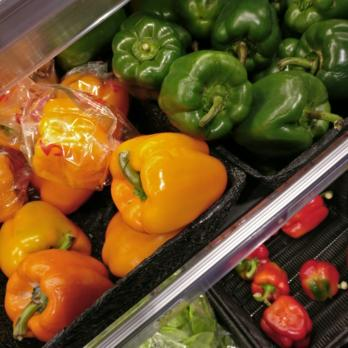
\includegraphics[width=13mm, height=13mm]{Chapter3/figures/decoded_iconic_images/Orange-Bell-Pepper_008.jpg} & 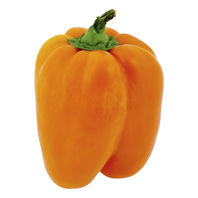
\includegraphics[width=13mm, height=13mm]{Chapter3/figures/iconic_image_figures/Orange-Bell-Pepper_Iconic.jpg} & 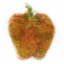
\includegraphics[width=13mm, height=13mm]{Chapter3/figures/decoded_iconic_images/vcca_xiwy/orange_bell_pepper_image2191.png}  \\[-0.7mm] 
		\hline \\[-3mm]
		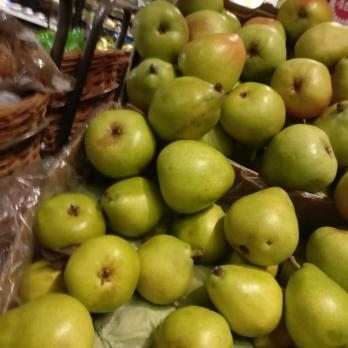
\includegraphics[width=13mm, height=13mm]{Chapter3/figures/decoded_iconic_images/Anjou_015.jpg} & 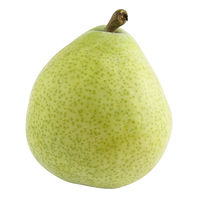
\includegraphics[width=13mm, height=13mm]{Chapter3/figures/iconic_image_figures/Anjou-Pear_Clean.jpg} & 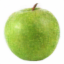
\includegraphics[width=13mm, height=13mm]{Chapter3/figures/decoded_iconic_images/vcca_xiwy/anjou_pear_image849.png} \\[-0.7mm]
		\hline
	\end{tabular}
	\vspace{-3mm}
	\captionsetup{width=.95\linewidth}
	\caption{Examples of decoded iconic images from VCCA$_{\vx \vi \vw \vy}$ with their corresponding natural image and true iconic image.}
	\vspace{-4mm}
	\label{fig:decoded_iconic_images}
\end{wrapfigure} 
\paragraph{Iconic Image Generation.} The iconic image decoder can be used for interpreting the outcomes of predicted classes. Figure \ref{fig:decoded_iconic_images} shows two examples of iconic images decoded from VCCA$_{\vx \vi \vw \vy}$ from two natural images of the classes \textit{Orange Bell Pepper} and \textit{Anjou Pear} from the test set. On the first row, %we see that 
the model has generated an iconic image of an orange-green colored bell pepper with the shape of the green bell pepper in its iconic image. On the second row, %we see that 
the decoded iconic image is a \textit{Granny Smith} apple instead of the true class \textit{Anjou Pear}. Hence, the iconic image decoder can be used as a tool for providing insights in why the classifier makes prediction errors. 




\vspace{-3mm}
\paragraph{Latent Space Visualizations.} The web-scraped iconic images and text descriptions structures the grocery items based on view-specific similarities in the latent space that are beneficial for fine-grained classification. Figure \ref{fig:latent_space_visualizations} demonstrates how adding either the iconic image $\vi$ or the text description $\vw$ can change the structure of the latent space. We used PCA for projecting the learned latent representations of the test set into a 2-dimensional space. We have plotted the corresponding iconic image for the latent representations of VAE$_{\vx}$, VCCA$_{\vx \vi}$, VCCA$_{\vx \vw}$ for visualization purposes in Figure \ref{fig:latent_space_visualizations}(a-c).  
The VAE$_{\vx}$ model in Figure \ref{fig:latent_space_visualizations}(a) separates raw and packaged grocery items into two separate clusters in the latent space. 
When adding the iconic image in in Figure \ref{fig:latent_space_visualizations}(b), we observe that the latent space becomes structured according to the color of the items. 
For VCCA$_{\vx \vw}$ in in Figure \ref{fig:latent_space_visualizations}(c), the latent space becomes structured according to the ingredients of the items, where we see in the raw grocery item cluster that bell peppers are placed in the upper region while apples are in the lower region. 

\begin{figure}[t]
	\centering
	
\begin{subfigure}[b]{0.3\textwidth}
	\centering
	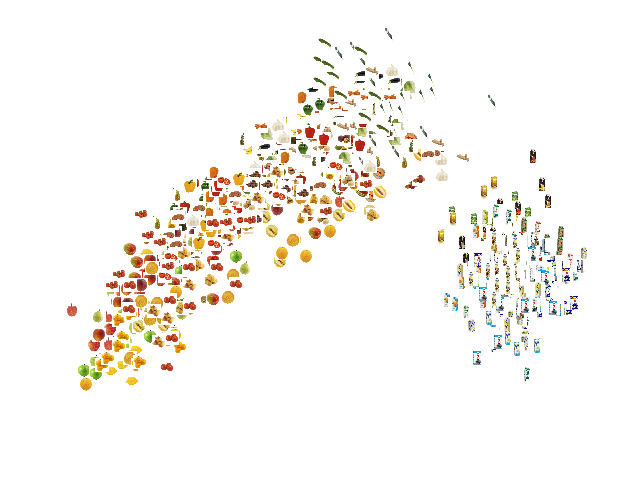
\includegraphics[width=\textwidth]{Chapter1/pics_paperB/pca_latents_vae_seed2}
	\vspace{-8mm}
	\caption{VAE$_{\vx}$}
	\label{fig:pca_latents_vae}
\end{subfigure}
\hfill
\begin{subfigure}[b]{0.3\textwidth}
	\centering
	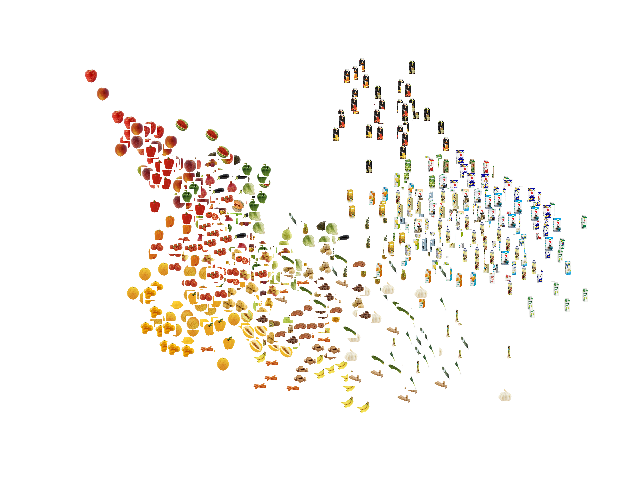
\includegraphics[width=\textwidth]{Chapter1/pics_paperB/pca_latents_vcca_xi_seed2}
	\vspace{-8mm}
	\caption{VCCA$_{\vx\vi}$}
\label{fig:pca_latents_vcca_xi}
\end{subfigure}
\hfill
\begin{subfigure}[b]{0.3\textwidth}
	\centering
	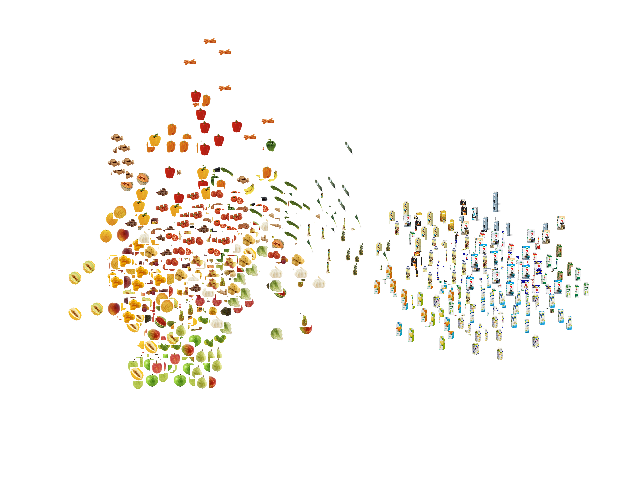
\includegraphics[width=\textwidth]{Chapter1/pics_paperB/pca_latents_vcca_xw_seed2}
	\vspace{-8mm}
	\caption{VCCA$_{\vx\vw}$}
\label{fig:pca_latents_vcca_xw}
\end{subfigure} \\ 
\begin{subfigure}[b]{0.3\textwidth}
	\centering
	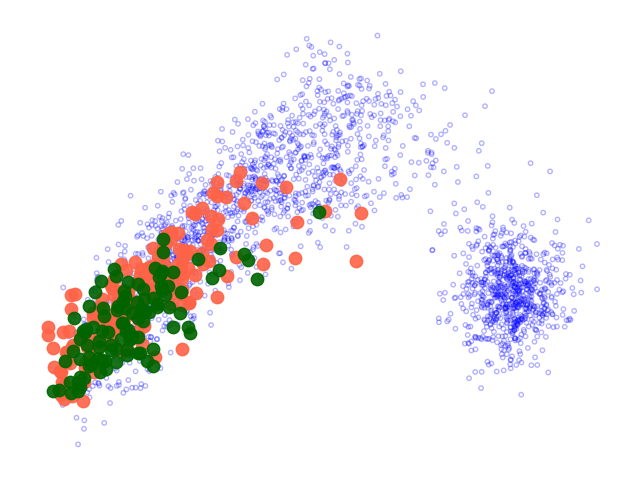
\includegraphics[width=\textwidth]{Chapter1/pics_paperB/pca_latents_apples_vae_seed2}
	\vspace{-8mm}
	\caption{VAE$_{\vx}$}
\label{fig:pca_latents_vae_apples}
\end{subfigure}
\hfill
\begin{subfigure}[b]{0.3\textwidth}
	\centering
	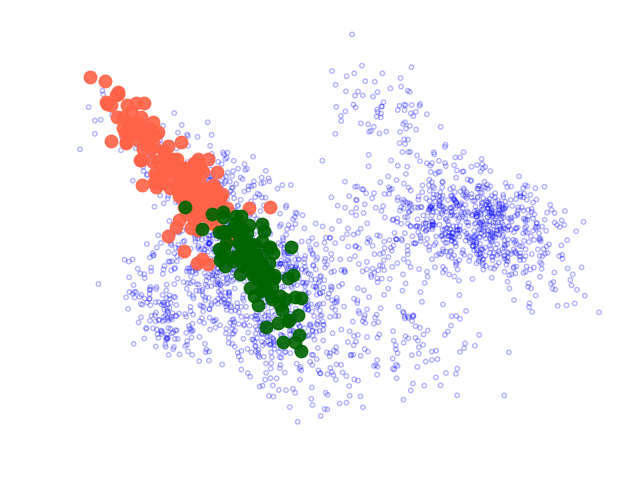
\includegraphics[width=\textwidth]{Chapter1/pics_paperB/pca_latents_apples_vcca_xi_seed2}
	\vspace{-8mm}
	\caption{VCCA$_{\vx\vi}$}
	\label{fig:pca_latents_vcca_xi_apples}
\end{subfigure}
\hfill
\begin{subfigure}[b]{0.3\textwidth}
	\centering
	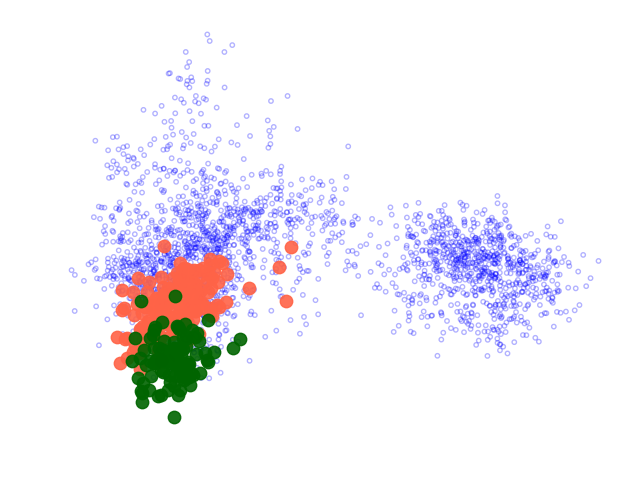
\includegraphics[width=\textwidth]{Chapter1/pics_paperB/pca_latents_apples_vcca_xw_seed2}
	\vspace{-8mm}
	\caption{VCCA$_{\vx\vw}$}
\label{fig:pca_latents_vcca_xw_apples}
\end{subfigure} \\
\begin{subfigure}[b]{0.3\textwidth}
	\centering
	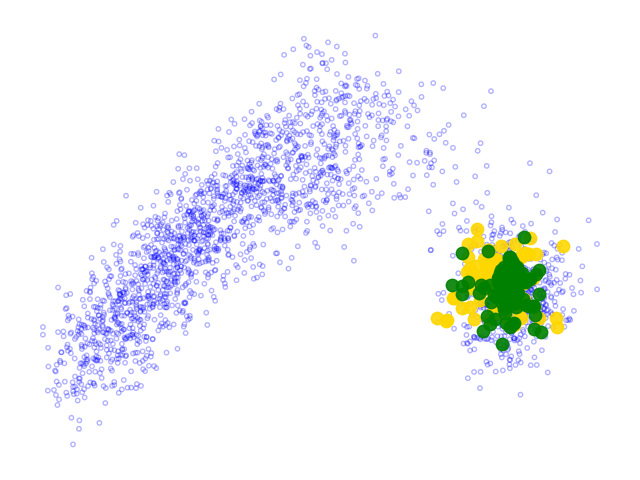
\includegraphics[width=\textwidth]{Chapter1/pics_paperB/pca_latents_juice_yoghurt_vae_seed2}
	\vspace{-8mm}
	\caption{VAE$_{\vx}$}
\label{fig:pca_latents_vae_juice_yoghurt}
\end{subfigure}
\hfill
\begin{subfigure}[b]{0.3\textwidth}
	\centering
	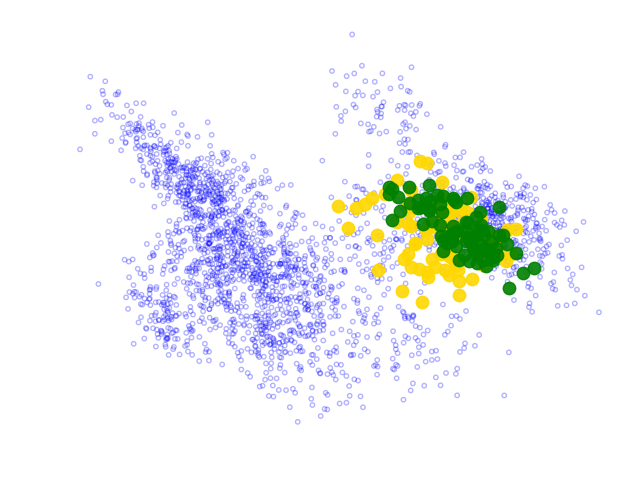
\includegraphics[width=\textwidth]{Chapter1/pics_paperB/pca_latents_juice_yoghurt_vcca_xi_seed2}
	\vspace{-8mm}
	\caption{VCCA$_{\vx\vi}$}
\label{fig:pca_latents_vcca_xi_juice_yoghurt}
\end{subfigure} 
\hfill
\begin{subfigure}[b]{0.3\textwidth}
	\centering
	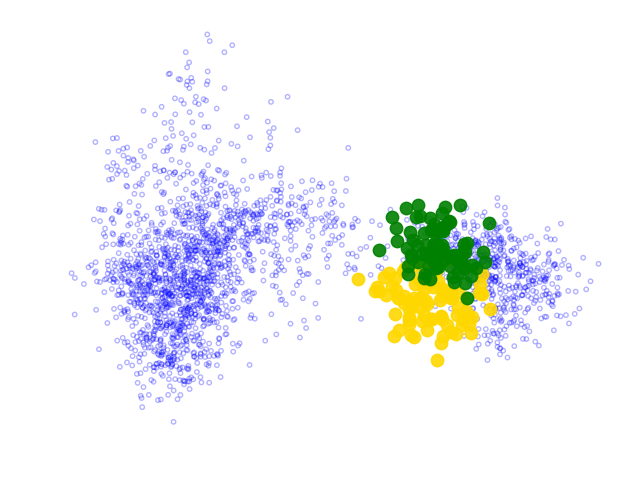
\includegraphics[width=\textwidth]{Chapter1/pics_paperB/pca_latents_juice_yoghurt_vcca_xw_seed2}
	\vspace{-8mm}
	\caption{VCCA$_{\vx\vw}$}
	\label{fig:pca_latents_vcca_xw_juice_yoghurt}
\end{subfigure}
	\vspace{-1mm}
	\caption{ Visualizations of the latent representations from VAE$_\vx$, VCCA$_{\vx\vi}$, and VCCA$_{\vx\vw}$ projected in 2-dimensional space with PCA. In (a-c), we show the latent representations plotted using the iconic images of the corresponding object class. In (d-f), we illustrate how the iconic images structures the items based on visual similarities by focusing on the \textcolor{ForestGreen}{green} and \textcolor{RedOrange}{red} apple classes in the dataset plotted in their corresponding colors. Similarly, in (g-i), we show how the text descriptions structure items based on ingredients and flavor by focusing on visually similar yoghurt (\textcolor{ForestGreen}{green}) and juice (\textcolor{GreenYellow}{yellow}) packages. The \textcolor{blue}{blue} dots correspond to all other grocery item classes. } 
	\label{fig:latent_space_visualizations}
	\vspace{-2mm}
\end{figure}

Next, we focus on a certain set of classes to gain more insights in how the web-scraped views affect the latent space. 
In Figure \ref{fig:latent_space_visualizations}(d-f), we inspect how items with different colors are separated in the latent space by utilizing $\vi$ or $\vw$ in VCCA by plotting the green and red apple classes as green and red points respectively. All other classes are plotted as smaller points in blue. We observe that both VCCA$_{\vx \vi}$ and VCCA$_{\vx \vw}$ manages to separate the apple classes better than VAE$_{\vx}$ where VCCA$_{\vx \vi}$ obtains the most clear separation.
We also want to inspect how the views separates visually similar items with different ingredients and flavors. Hence, in Figure \ref{fig:latent_space_visualizations}(g-i), we have plotted  white-colored yoghurt and juice package classes in the colors green and yellow respectively. 
We see that VCCA$_{\vx \vw}$ manages to separate these items better than VCCA$_{\vx \vw}$ due to different ingredient information about yoghurt and juice that is mentioned in the text descriptions. 


%\paragraph{Visualization of Latent Space.} The web-scraped iconic images and text descriptions structures the grocery items based on view-specific similarities in the latent space that are beneficial for fine-grained classification. In Figure \ref{fig:latent_space_visualizations}, we illustrate how adding either the iconic image $\vi$ or the text description $\vw$ changes the structure of the latent space, where we have used PCA to project the latent representations into a 2-dimensional space. In Figure \ref{fig:latent_space_visualizations}(a-c), we have plotted the corresponding iconic image for all latent representations of models VAE$_{\vx}$, VCCA$_{\vx \vi}$, VCCA$_{\vx \vw}$ for visualization purposes. The latent space for VAE$_{\vx}$ separates raw and packaged grocery items into two separate clusters. When adding the iconic image in VCCA$_{\vx \vi}$, we observe that the latent space becomes structured according to the color of the items. For VCCA$_{\vx \vw}$, the latent space becomes structured according to the ingredients of the items, where we see in the raw food cluster that bell peppers are placed in the upper region while apples are in the lower region. 

%Next, we focus on a certain set of classes to inspect to gain more insights in how the additional data views affect the latent space. First, we focus on the green and red apples classes to inspect how the views handle visually different items in color. In Figure \ref{fig:latent_space_visualizations}(d-f), we plot the latent representations for the three models but highlight the green and red apple classes by plotting them as green and red dots respectively. All other classes are plotted as smaller blue dots. We see that both VCCA$_{\vx \vi}$ and VCCA$_{\vx \vw}$ manages to separate the apple classes better than VAE$_{\vx}$, where adding the iconic images yields the most clear separation. Next, we want to study the benefits of the text descriptions. We focus on some yoghurt and juice package classes that are visually similar but have very different ingredients and flavors. In Figure \ref{fig:latent_space_visualizations}(g-i), we plot the latent representations for the three models again where the yoghurt and juice classes are plotted in green and yellow colored dots respectively. Here, we see that VCCA$_{\vx \vw}$ manages to separate these items better than VCCA$_{\vx \vw}$ due to the differences in the text descriptions between the selected package classes. 



%Conclusions on visualizations: ​

%Iconic image structures items based on visual similarities​

%Text description structures items based on ingredients and flavor



%\paragraph{Iconic Image Generation.} The iconic image decoder can provide explanations for the predicted classes. Figure \ref{fig:decoded_iconic_images} shows two examples of decoded iconic images from two natural images where the class labels are \textit{Orange Bell Pepper} and \textit{Anjou Pear}. On the first row, we see that VCCA$_{\vx \vi \vw \vy}$ has recognized the green bell peppers in the natural image and generated a mixed orange and green bell pepper in the iconic image. On the second row, we see that the decoded iconic image is a \textit{Granny Smith} apple instead of a pear which was the true class. The classifier consequently predicts the natural image to be a \textit{Granny Smith} apple. Hence, the iconic image decoder can be used as a tool for providing an intuition of why the classifier made an error. 



\section{Discussion}\label{chap3:sec:discussion}

In this chapter, we summarized the contributions in Paper \ref{paperA} and \ref{paperB} on FGIR for assisting VI people with grocery shopping using an assistive vision app on their mobile phone. In Paper \ref{paperA}, we collected a publicly available dataset with mobile phone images of groceries taken in grocery stores as well as web-scraped information about the items from a supermarket website. In Paper \ref{paperB}, we show how the web-scraped information can be multi-view learning can be used for use the web-scraped information to train more accurate and robust image classifiers. More specifically, the iconic images structures the items after visual similarities such as colors and shapes in the learned latent space, while the text descriptions pushes items with similar ingredients and flavors closer to each other.
This shows that the cheap-to-collect web-scraped views can serve as a good alternative for improving the fine-grained classification performance instead of collecting more natural images in the grocery stores. 

Regarding the dataset collection in Paper \ref{paperA}, we have some belated suggestions on how to make the collection procedure easier and also how to enrich the dataset. The images should be collected by recording videos of the grocery items rather than taking still images in the grocery stores. This would potentially enhance the dataset size and could also mitigate the class imbalance in the training and test splits. Furthermore, we could evaluate the classifiers on video sequences which would be a more realistic and user-friendly setting for how an assistive vision app would be used by VI people. Another suggestion to enrich the dataset would be to download more instances of iconic images and text descriptions from supermarket websites, which could potentially allow the VCCA model to capture the view-specific variations into the learned latent representations. Finally, it would have been valuable to have natural images collected by VI people to benchmark the classifiers on scenarios with the actual target users~\cite{jayant2011supporting,massiceti2021orbit}. 

In Paper \ref{paperB} and Section \ref{chap3:sec:experiments}, we observed that utilizing the iconic images in VCCA affects the classification performance significantly better than the text descriptions. We believe that this could be due to the noise in the text descriptions where often there are only a few words that are relevant to the image recognition task. In the future, we could pre-process the text descriptions by removing stop words, e.g., 'the', 'it', 'and', etc., and other words that are irrelevant for recognizing the fine-grained details of the items. Moreover, we could use pretrained word embeddings~\cite{mikolov2013distributed, pennington2014glove, lan2019albert} for considering word similarities, add attention mechanisms~\cite{luong2015effective, vaswani2017attention} in the model for focusing on relevant words, and use data augmentation techniques for text~\cite{wei2019eda} to learn more robust joint latent representations. 

Finally, we believe the Grocery Store dataset could be used for benchmarking image classifiers on zero/few-shot learning~\cite{xian2018zero, wang2020generalizing} and continual learning~\cite{delange2021continual, parisi2019continual} settings. 
This would be an important extension of the dataset as these applications are crucial to enhance the usability of assistive vision systems in real-world scenarios. 


%In the experiments, we showed that utilizing the web-scraped information with VCCA can enhance the performance of grocery item classifiers. This shows that the cheaper web-scraped views can serve as a good alternative for improving classification performance over collecting more natural images in the grocery stores. Furthermore, we illustrated how the iconic images and text descriptions affects the structure of the latent space based on view-specific information. More specifically, the iconic images structures the latent space after visual similarities such as colors and shapes, while the text descriptions pushes items with similar ingredients and flavors closer to each other in the latent space. Finally, we demonstrated how the iconic images can be used for providing potential explanations for misclassifications, which could help us detect hard classes and give us indications of how robust the latent representations are to classifying images with different classes. 

%We observed that utilizing the iconic images in VCCA affects the classification performance significantly better than the text descriptions. Potentially, this is due to the text description view to be more noisy than the iconic images as there are few words that are relevant to the recognition task. However, the text descriptions could be utilized more efficiently, for example by pre-processing the text to keep words describing fine-grained details about the items as well as removing stop words ('the', 'it', 'and', etc.) and other irrelevant words. A second option would be to use attention mechanisms~\cite{luong2015effective, vaswani2017attention} that helps the model to learn which words to emphasize on when learning the joint latent representations. We could also encode the text into a single-vector embedding with various methods~\cite{mikolov2013distributed, pennington2014glove, lan2019albert} and replace the RNN with an MLP predicting in the embedding space which the text embedding the natural image is closes to. 

%% Paper on Text augmentation: https://arxiv.org/abs/1901.11196

%Regarding the dataset collection, we have suggested extensions on how to provide more useful information about the items to improve the recognition task. Firstly, it would be valuable to download instances of iconic images and text descriptions from more supermarket websites to potentially allow the VCCA model to capture more view-specific variations into the learned representations. Secondly, the model should be extended to handle video data rather than still images. This would require record videos with the mobile phone camera in the grocery stores to properly evaluate the classifiers. Nevertheless, the extension to video would be beneficial for user experience of the recognition app since the classifier would receive more chances to classify the items correctly by utilizing multiple frames. 

%Finally, the Grocery Store dataset could be extended to zero/few-shot learning~\cite{xian2018zero, wang2020generalizing} and continual learning~\cite{delange2021continual, parisi2019continual} settings. Such applications are important for assistive vision devices to build data-efficient and adaptable systems that improves their usability in real-world scenarios. 



